
\section{One-Way Analysis of Variance Methods}

\par In the previous section, we found a significant race-based difference in the ages of deadly force victims between two racial categories, white and nonwhite. In the parametric setting, we could extend our analysis to more than two categories using a one-way analysis of variance (ANOVA) model, then make comparisons between each difference with Tukey's honest significant differences (HSD). This section explores the analogous distribution-free tests: the Kruscal-Wallis test for unequal treatment effects, and the Steel, Dwass, Critchlow-Fligner multiple comparisons procedure.

\subsection{Age vs. Race: Parametric Analysis}

\begin{table}[h]
    \centering
    \begin{tabular}{|c|c|c|c|c|}
        \hline
        ``White" & ``Black" & ``Hispanic/Latino" & ``Asian/Pacific Islander" & ``Native American"\\
        229 & 131 & 64 & 10 & 4\\
        \hline
    \end{tabular}
    \caption{Observation counts for the five levels of $raceethnicity$}
    \label{tab:raceethnicity_levels_n}
\end{table}

\par Table \ref{tab:raceethnicity_levels_n} shows the count of observations for the five levels of $raceethnicity$. The last two groups have only 10 and 4 observations, respectively, making them too much smaller than the other three for valid comparisons. Thus we drop observations coded ``Asian/Pacific Islander" and ``Native American" and compare the remaining three.

\begin{figure}[h]
    \centering
    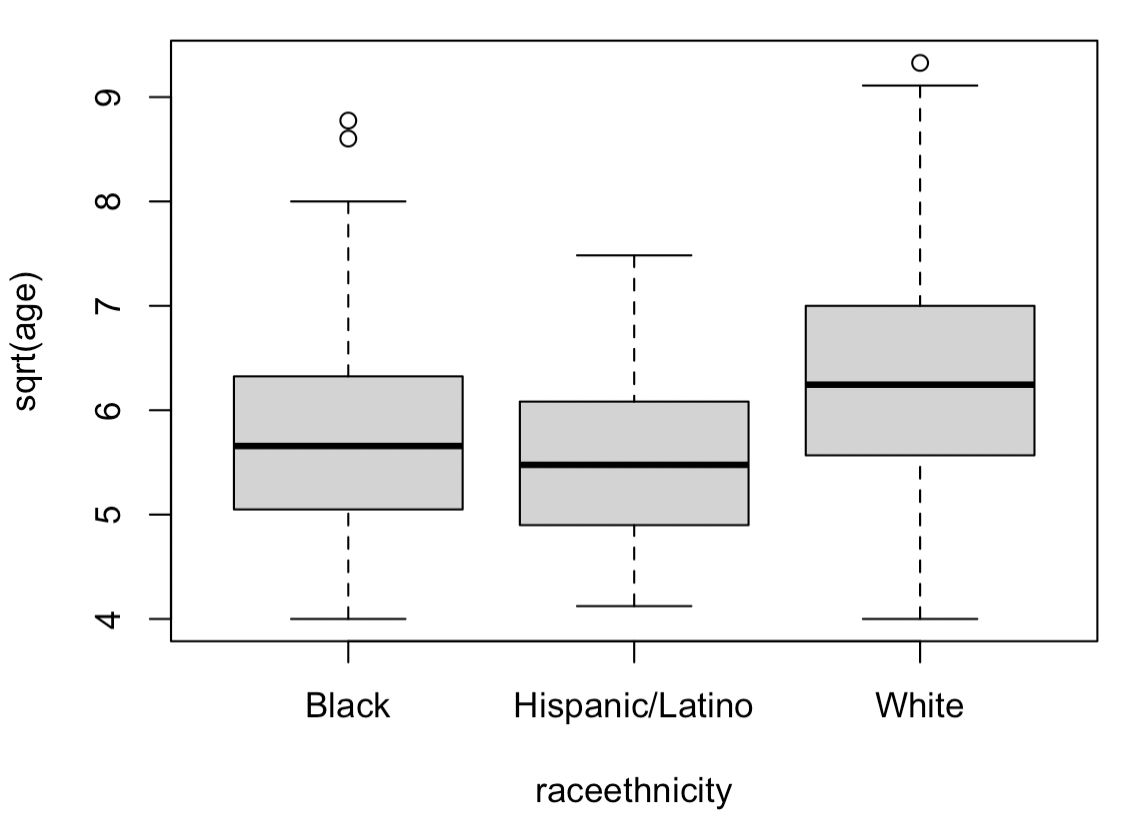
\includegraphics[scale=.4]{boxplot_sqage_raceethnicity.png}
    \caption{Box plots of $\sqrt{age}$ vs. three levels of $raceethnicity$}
    \label{fig:aov1_boxplots}
\end{figure}

\par We see in Figure \ref{fig:aov1_boxplots} that the median $\sqrt{age}$ of white victims looks significantly higher than for both Black and Latino victims. Using the base R function \texttt{aov()}, we fit an ANOVA model to the data and obtain a $p$-value of $4.273*10^{-9}$. If this test were valid, we would conclude quite confidently that at least one of the treatment effects $\tau_{W}, \tau_{B}, \tau_{L}$ is not equal to the rest.

\par \bigskip We would then proceed with a multiple comparisons procedure, such as Tukey's HSD. Using the base R function \texttt{TukeyHSD()}, we obtain intervals for the three configurations of differences in means, adjusted for differences in variance, with 95 percent overall confidence. As shown in Table \ref{tab:aov1_results}, Tukey's HSD claims that, on average, white victims are older than both Black and Latino victims.

\par \bigskip These distribution-reliant claims ring hollow when we check their conditions for inference. Shown in Figure \ref{fig:aov1_plots}, the residuals appear to have different-sized variances for the three groups and lift up considerably from the tails of the expected normal distribution. The picture gets more complicated when we conduct statistical tests: though Levene's test returns a $p$-value of .0243, the Anderson-Darling test yields a $p$-value of 0.0564, which rejects the null hypothesis of normality only at a weak significance level of 0.1. We may consider the ANOVA model somewhat more meaningful in this case, but our distribution-free methods will give us much more robust conclusions.

\vspace{.2in}

\begin{figure}[h]
    \centering
    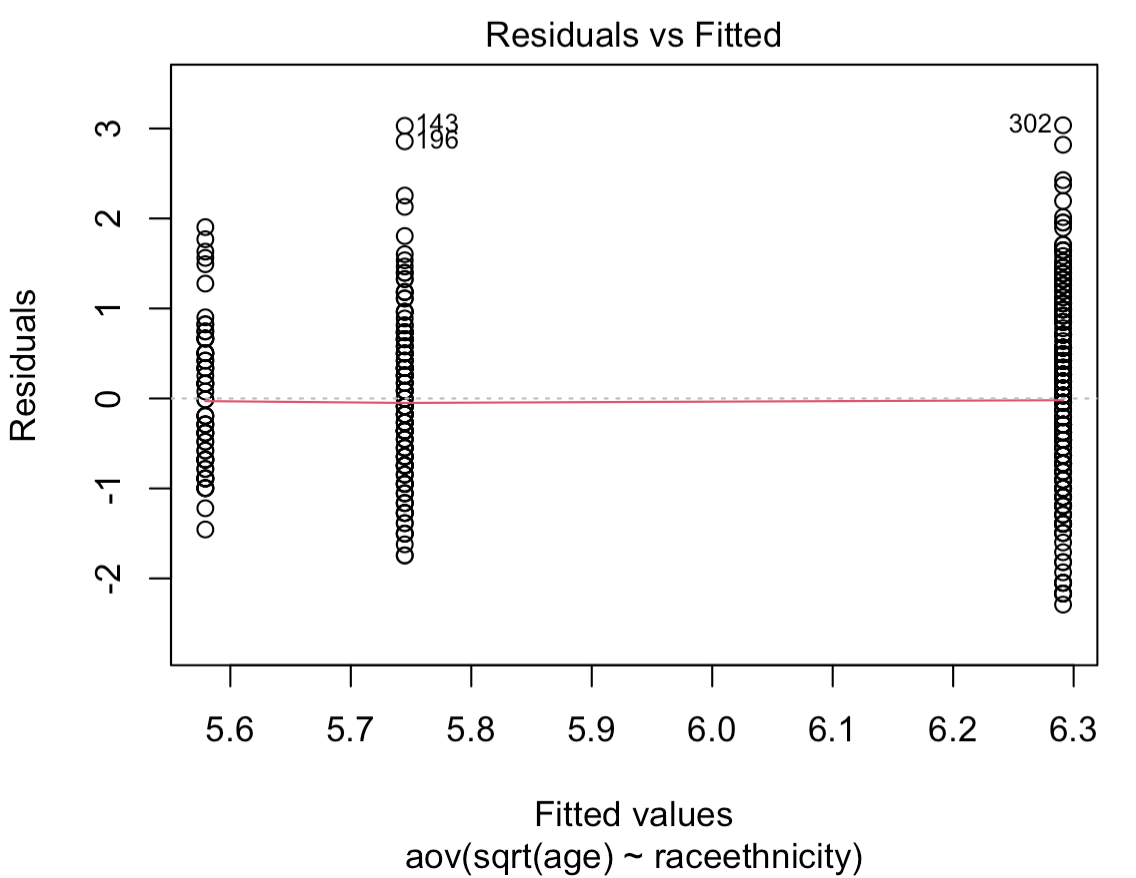
\includegraphics[scale=.35]{aov1_plot1.png}
    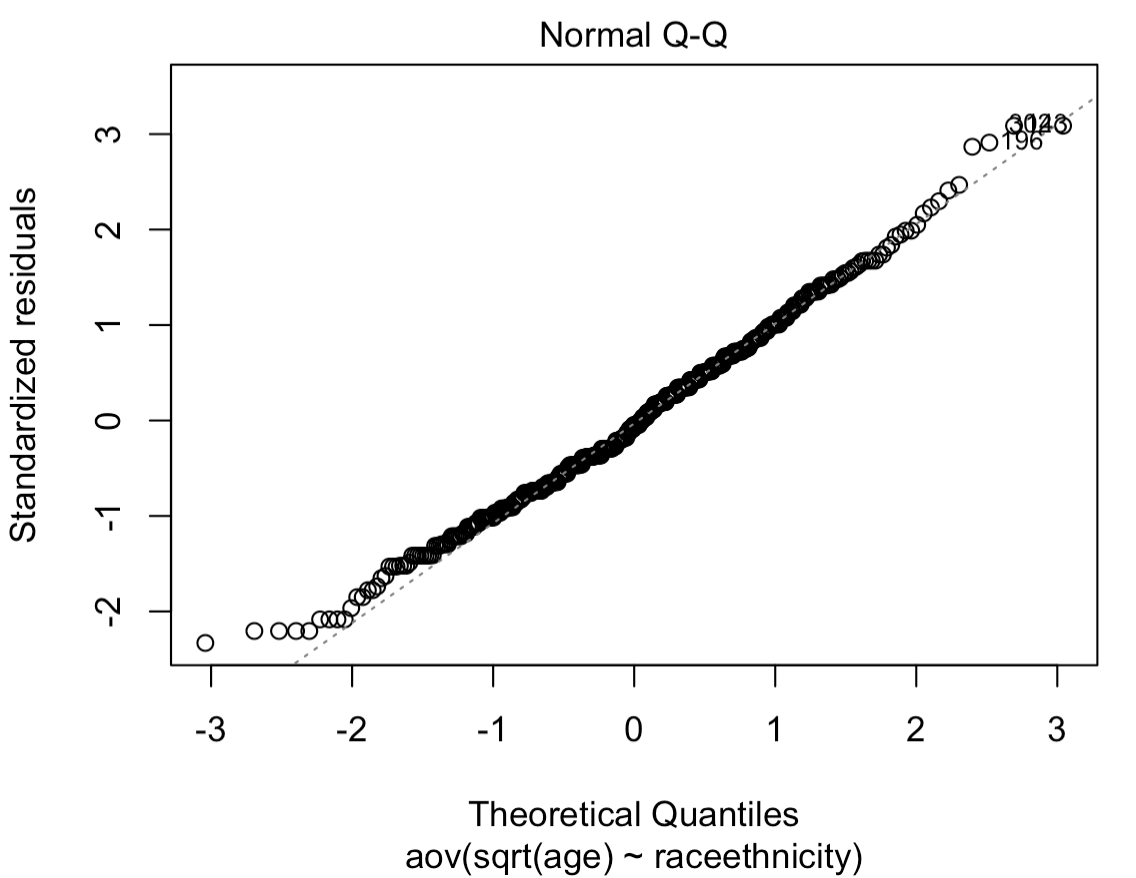
\includegraphics[scale=.35]{aov1_plot2.png}
    \caption{Diagnostic plots for the ANOVA model of $age$ vs. $raceethnicity$}
    \label{fig:aov1_plots}
\end{figure}

\subsection{Age vs. Race: Nonparametric Analysis}

\par Turning to our nonparametric toolbox, we apply the Kruscal-Wallis test, which ranks the combined samples to measure whether the observations in at least one of them are generally ranked higher or lower than those of the other two samples. This test assumes the populations of interest have equal variance, so its results are questionable considering the rejection of the null hypothesis of Levene's test. That said, it is much more resilient to unequal variance than the ANOVA model, so its conclusions are more robust. We will once again perform this rank-based test on the untransformed $age$ variable and use the LSA to reduce computing time.

\newpage

\textbf{Kruscal-Wallis test}

\bigskip $H_0: \tau_{W} = \tau_{B} = \tau_{L}$

$H_1:$ Not all $\tau_k$ equal, $k \in \{W,B,L\}$ \hspace{.5in} Reject $H_0$ if $H^{\prime} \ge \chi^2_{2,\alpha}$.

\par \bigskip Using the R function \texttt{pKW()} from the package \texttt{NSM3}, we find that $H^{\prime} = 37.515$ and obtain a $p$-value of $7.140*10^{-9}$. We reject the null hypothesis and conclude that at least one of the three groups has a different median age than at least one of the others. Note that the Kruscal-Wallis $p$-value is only marginally higher than that of the ANOVA model, and both firmly reject the null hypothesis.

\par \bigskip Our conclusion from the Kruscal-Wallis test motivates us to identify significant pairwise differences with the Steel-Dwass-Critchlow-Fligner procedure, which applies the rank sum test to the three configurations of combined pairs of populations while maintaining overall confidence of $1-\alpha$.

\bigskip \textbf{Steel, Dwass, Critchlow-Fligner procedure}

\bigskip For each pair $(\tau_u,\tau_v)$, decide $\tau_u \not= \tau_v$ if $|W^*_{uv}| \ge w^*_{\alpha}$.

\par \bigskip Using the R function \texttt{pSDCFlig()} from the package \texttt{NSM3}, we obtain the three statistics $W^*_{uv}$ and use the LSA. Based on its results (shown in Table \ref{tab:aov1_results}), we decide with 95 percent overall confidence that white victims have a different median age than Black and Latino victims. We can now use a procedure devised by Spjøtvoll to find adjusted Hodges-Lehmann estimators for each difference in group medians. Using custom R code, we obtain the estimates $\hat{\theta}_{WB} = 6.849$ and $\hat{\theta}_{WL} = 8.309$; the estimate $\hat{\theta}_{BL} = 1.460$ is not significant. Finally, from the ordered differences of each population, we find three intervals for the true median with 95 percent overall confidence.

\par \bigskip The results of this subsection are summarized in Table \ref{tab:aov1_results}. We see that our nonparametric methods yield $p$-values that are about twice the size of the parametric $p$-values, except for the test of $\theta_{BL}$, which is slightly smaller than its distribution-based counterpart. That said, every conclusion is quite strong in this case, and the outcomes of the two types of tests are no different. 

\vspace{.2in}

\begin{table}[h]
    \centering
    \begin{tabular}{|l|c|c|c|c|}
        \hline
        \textbf{parameter} & \textbf{procedure} & \textbf{p-value} & \textbf{estimate} & \textbf{95 pct. CI}\\
        \hline
        General & one-way ANOVA & $4.273*10^{-9}$ & -- & --\\
        differences & Kruscal-Wallis & $7.140*10^{-9}$  & -- & --\\
        \hline
        $\theta_{WB}$ & Tukey's HSD & 0.0000019 & $\hat{\mu}_{WB} = 6.577$ & $(3.595, 9.430)$\\
        & SDCFlig & 0.0000038 & $\hat{\theta}_{WB} = 6.849$ & $(4.000, 10.000)$\\
        \hline
        $\theta_{WL}$ & Tukey's HSD & 0.0000015 & $\hat{\mu}_{WL} = 8.452$ & $(4.687, 12.001)$\\
        & SDCFlig & 0.0000022 & $\hat{\theta}_{WL} = 8.309$ & $(5.000, 12.000)$\\
        \hline
        $\theta_{BL}$ & Tukey's HSD & 0.5137 & $\hat{\mu}_{BL} = 1.874$ & $(-2.132, 5.521)$\\
        & SDCFlig & 0.4601 & $\hat{\theta}_{BL} = 1.460$ & $(-2.000, 5.000)$\\
        \hline
    \end{tabular}
    \caption{Results for $age$ vs. $raceethnicity$}
    \label{tab:aov1_results}
\end{table}

\newpage

\subsection{More One-Way Analysis}

We proceed with three additional analyses of treatment effects with the same methods.

\begin{figure}[h]
    \centering
    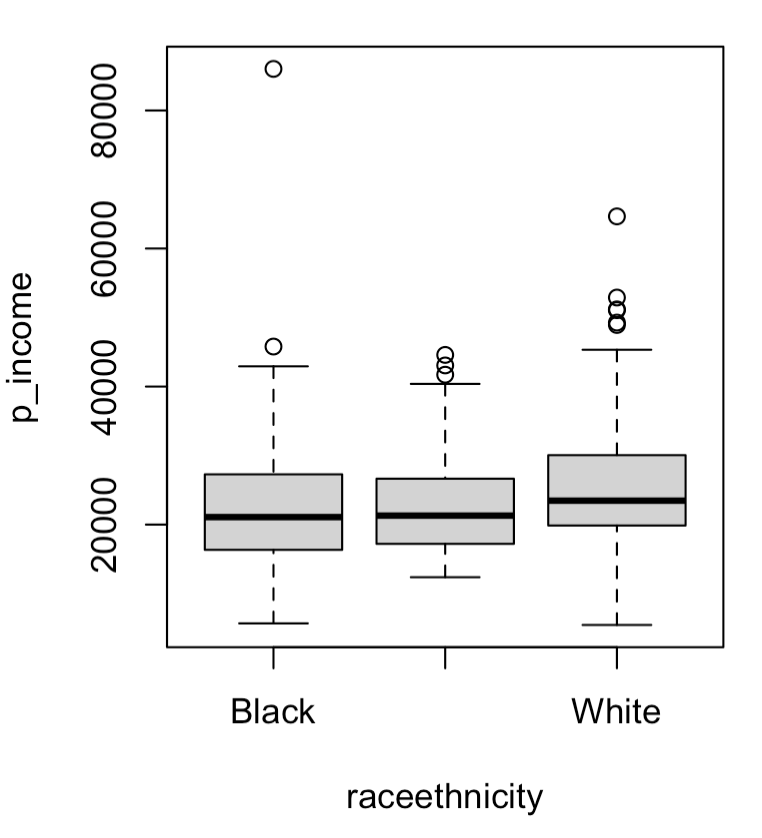
\includegraphics[scale=.35]{boxplot_pincome_race.png}
    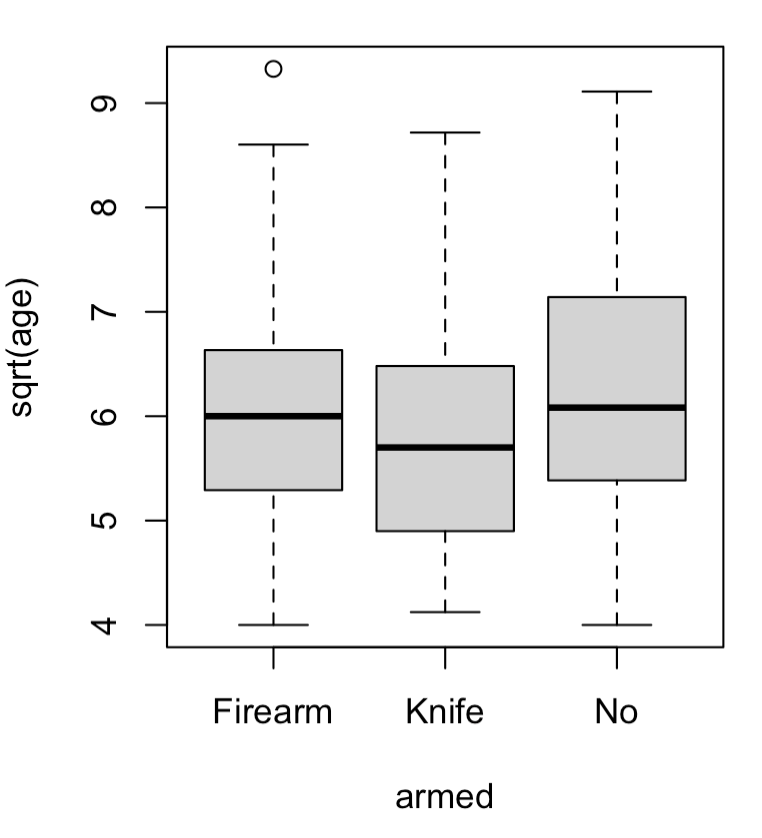
\includegraphics[scale=.35]{boxplot_age_armed.png}
    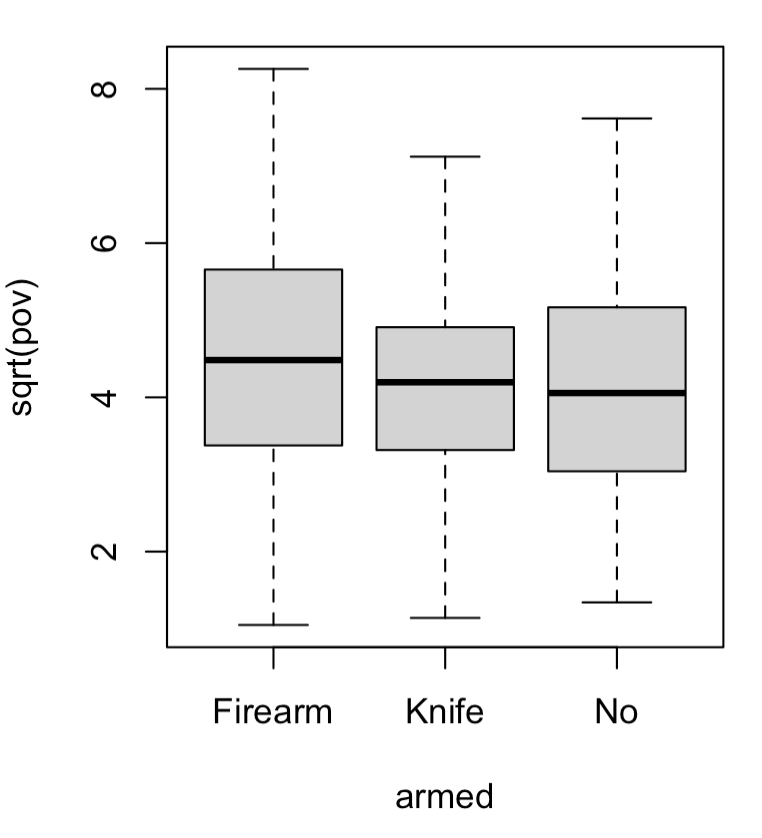
\includegraphics[scale=.35]{boxplot_pov_armed.png}
    \caption{Box plots of $\sqrt{p\_income}$ vs. $raceethnicity$, and of $\sqrt{age}$ and $\sqrt{pov}$ vs. $armed$}
    \label{fig:aov234_boxplots}
\end{figure}

Results for the analysis of $p\_income$ against $raceethnicity$ are summarized in Table \ref{tab:aov2_results}. In this case, Levene's test yields a large $p$-value of 0.417, while Anderson-Darling strongly rejects normality of residuals. The square root transformation is found to worsen variance, so the untransformed model is used this time. Interestingly, the conclusions of our nonparametric tests are considerably stronger than those of our (invalid) parametric tests. The SDCFlig procedure even identifies a significant difference between median age for white vs. Latino victims, which Tukey's HSD does not.

\begin{table}[h]
    \centering
    \begin{tabular}{|l|c|c|c|c|}
        \hline
        \textbf{parameter} & \textbf{procedure} & \textbf{p-value} & \textbf{estimate} & \textbf{95 pct. CI}\\
        \hline
        General & one-way ANOVA & 0.02071 & -- & --\\
        differences & Kruscal-Wallis & 0.0021  & -- & --\\
        \hline
        $\theta_{WB}$ & Tukey's HSD & 0.0428 & $\hat{\mu}_{WB} = 2369.67$ & $(60.56, 4678.77)$\\
        & SDCFlig & 0.0065 & $\hat{\theta}_{WB} = 2657.40$ & $(608.00, 4623.00)$\\
        \hline
        $\theta_{WL}$ & Tukey's HSD & 0.1046 & $\hat{\mu}_{WL} = 2581.70$ & $(-398.68, 5562.09)$\\
        & SDCFlig & 0.0301 & $\hat{\theta}_{WL} = 2520.99$ & $(186.00, 4816.00)$\\
        \hline
        $\theta_{BL}$ & Tukey's HSD & 0.5137 & $\hat{\mu}_{BL} = 212.04$ & $(-3002.64, 3426.71)$\\
        & SDCFlig & 0.9852 & $\hat{\theta}_{BL} = 136.41$ & $(-2747.00, 2529.00)$\\
        \hline
    \end{tabular}
    \caption{Results for $age$ vs. $raceethnicity$}
    \label{tab:aov2_results}
\end{table}

\newpage

\par Our final two analyses involve the categorical variable $armed$. As before, we trim the data to only include the three levels of $armed$ with the most observations. In the resulting dataset, there are 100 unarmed victims, 219 firearm-wielding victims, and 66 knife-wielding victims.

\par \bigskip Table \ref{tab:aov3_results} displays the results of our analysis of $age$ against $armed$. Levene's test again does not reject its null hypothesis for these groups, while the Anderson-Darling test does. The outcomes of the parametric and nonparametric tests in this case are quite similar. One notable difference is that Tukey's HSD returns a much higher $p$-value for $\theta_{FK}$ than for $\theta_{UF}$, while the Kruscal-Wallis $p$-values for those two differences are virtually the same. Perhaps the upper-tailed outliers of age for the firearm- and knife-wielding groups (seen in the second plot in Figure \ref{fig:aov234_boxplots}) make the parametric methods consider those two distributions closer to each other than to the unarmed group.

\vspace{.2in}

\begin{table}[h]
    \centering
    \begin{tabular}{|l|c|c|c|c|}
        \hline
        \textbf{parameter} & \textbf{procedure} & \textbf{p-value} & \textbf{estimate} & \textbf{95 pct. CI}\\
        \hline
        General & one-way ANOVA & 0.0914 & -- & --\\
        differences & Kruscal-Wallis & 0.0796  & -- & --\\
        \hline
        $\theta_{UF}$ & Tukey's HSD & 0.1620 & $\hat{\mu}_{UF} = 2.852$ & $(-0.820, 6.524)$\\
        & SDCFlig & 0.3590 & $\hat{\theta}_{UF} = 2.000$ & $(-2.000, 6.000)$\\
        \hline
        $\theta_{UK}$ & Tukey's HSD & 0.0905 & $\hat{\mu}_{UK} = 4.313$ & $(-0.512, 9.139)$\\
        & SDCFlig & 0.0803 & $\hat{\theta}_{UK} = 4.000$ & $(0.000, 9.000)$\\
        \hline
        $\theta_{FK}$ & Tukey's HSD & 0.7004 & $\hat{\mu}_{FK} = 1.461$ & $(-2.811, 5.734)$\\
        & SDCFlig & 0.3239 & $\hat{\theta}_{FK} = 2.000$ & $(-2.000, 6.000)$\\
        \hline
    \end{tabular}
    \caption{Results for $age$ vs. $armed$}
    \label{tab:aov3_results}
\end{table}

\par Lastly, Table \ref{tab:aov4_results} summarizes results for our analysis of $pov$ against $armed$. The $p$-value of Levene's test is an indecisive 0.05415, but the Anderson-Darling test strongly rejects normality, as usual. Across the board, our distribution-free methods are less confident in rejection than our distribution-based methods. Both ANOVA and the Kruscal-Wallis test reject the null only at levels .1 and above.

\begin{table}[h]
    \centering
    \begin{tabular}{|l|c|c|c|c|}
        \hline
        \textbf{parameter} & \textbf{procedure} & \textbf{p-value} & \textbf{estimate} & \textbf{95 pct. CI}\\
        \hline
        General & one-way ANOVA & 0.0672 & -- & --\\
        differences & Kruscal-Wallis & 0.081 & -- & --\\
        \hline
        $\theta_{UF}$ & Tukey's HSD & 0.1874 & $\hat{\mu}_{UF} = -2.682$ & $(-6.283, 0.919)$\\
        & SDCFlig & 0.2043 & $\hat{\theta}_{UF} = 2.470$ & $(-6.000, 0.900)$\\
        \hline
        $\theta_{UK}$ & Tukey's HSD & 0.8364 & $\hat{\mu}_{UK} = 1.145$ & $(-3.587, 5.877)$\\
        & SDCFlig & 0.9754 & $\hat{\theta}_{UK} = 0.530$ & $(-3.400, 4.600)$\\
        \hline
        $\theta_{FK}$ & Tukey's HSD & 0.0815 & $\hat{\mu}_{FK} = 3.827$ & $(-0.363, 8.012)$\\
        & SDCFlig & 0.1456 & $\hat{\theta}_{FK} = 3.000$ & $(-0.700, 7.200)$\\
        \hline
    \end{tabular}
    \caption{Results for $pov$ vs. $armed$}
    \label{tab:aov4_results}
\end{table}